%!TEX root = ../proyecto.tex
\chapter{Modelos de Soft Computing considerados.}
\section{Mapas auto-organizados \textit{(Self Organizing Map)}}
A principio de la década de los 80 el científico finlandés Teuvo Kohonen \cite{kohonensom} planteó un modelo de aprendizaje automático no supervisado y competitivo basándose en el estudio del funcionamiento del córtex cerebral. El modelo planteado, denominado mapa auto-organizado, red auto-organizada o red neuronal de Kohonen, entre otros nombres similares, es una red neuronal artificial, y las principales características que la definen son las siguientes:\\

\begin{itemize}
	\item Es una \textbf{red neuronal artificial}. Esto quiere decir, a grandes rangos, que la estructura que genera el modelo está basada en una red de múltiples unidades llamadas ``neuronas'' que se encuentra interconectadas.
	
	\item La red neuronal de Kohonen tiene \textbf{dos capas}. Una capa de entrada, con tantas neuronas como características tenga una muestra a ser evaluada por la red, y una capa de salida de un tamaño que decide el usuario. Habitualmente, esta capa de salida, también llamada capa competitiva o capa de Kohonen, presenta una distribución bidimensional, aunque podría perfectamente usarse cualquier otro número de dimensiones.

	\item Cada neurona de la capa de entrada está asociada con todas las neuronas de la capa de salida y las neuronas de la capa de salida no están interconectadas entre sí. A este tipo de red neuronal, en la que no existen ciclos, se le denomina \textbf{red neuronal pre-alimentada} \textit{(feed-forward)}.

	\item Asociada a cada neurona de la capa de salida, tenemos un vector de pesos sinápticos obtenido a través de las conexiones con la capa de entrada que es modificado durante el proceso de aprendizaje. A dicho vector de pesos se le llama vector de referencia y representa el valor promedio de la categoría asociada a esa neurona. El conjunto de todos esos vectores de referencia es denominado \textit{codebook}.

	\item Es un algoritmo \textbf{no supervisado} capaz de encontrar patrones comunes basándose en los datos de la muestra de entrada sin necesidad de que cuando una muestra entre a la red se indique a qué categoría pertenece.

	\item Es un modelo \textbf{competitivo}. Cuando se recibe una muestra todas las neuronas compiten por ser activadas pero sólo la mejor será activada.
\end{itemize}

\begin{figure}
\centering
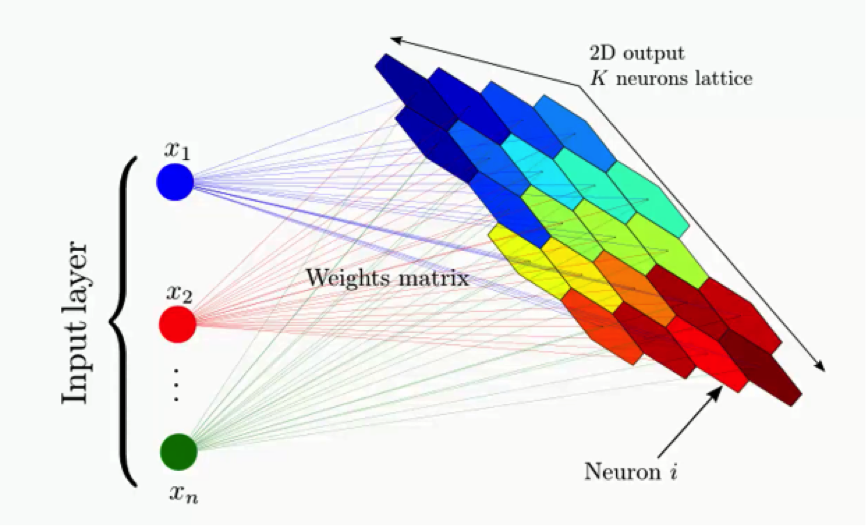
\includegraphics[width=0.8\textwidth]{imagenes/arquitectura_som.png}

\caption{Esquema de una red neuronal de Kohonen.}
%\textit{Autor: Damian Jankowski}
\end{figure}

\subsection{Proceso de entrenamiento.}

En primer lugar, se \textbf{inicializan} \textbf{los pesos} asociados a la capa de salida. Lo más habitual, es tomar dichos pesos de una distribución aleatoria.
Para un correcto funcionamiento dichos pesos deben estar normalizados entre 0 y 1. En nuestro caso, hemos tomado los pesos de una distribución aleatoria uniforme en el intervalo $[0, 1)$.\\

El proceso de entrenamiento que se presenta a continuación \textbf{se repite hasta que se alcanza el número de iteraciones máximo}, determinado por el parámetro $\lambda$. La variable $t$ representa cada una de las iteraciones.\\

Después, para cada una de las muestras, $X$, sacadas de la distribución de muestras, de forma aleatoria, se realizan los siguientes pasos: \\\\
1 - Se \textbf{calcula la distancia euclídea} entre la muestra $X$ y cada una de las neuronas de la capa de salida. También se pueden utilizar otro tipo de distancias.\\
$$distancia(X) = || W - X ||$$\\
2 - Se \textbf{busca la neurona que ha obtenido una menor distancia}. Esta neurona es considerada la neurona ganadora o BMU \textit{(Best Matching Unit)}.\\
$$BMU_X = argmin_{W_{i, j}} \; distancia(X) = argmin_{W_{i, j}} || W - X ||$$\\

La función \textit{argmin} devuelve el índice del array en el que se alcanza el valor mínimo.

3 - Se realiza un \textbf{proceso de actualización de las matrices de pesos} en base a lo obtenido anteriormente, según la siguiente fórmula.\\
$$ W_{i, j}^{(t+1)} = W_{i, j}^{(t)} + \Delta {W_{i,j}} $$\\

La actualización depende tanto de la distancia de la muestra al vector de pesos como de otros dos parámetros: la tase de aprendizaje y una función de vecindario.\\

$$\Delta W_{i,j} = \eta(t)\delta_f(i,j)(X-W_{i,j})$$\\

La función $\delta_f(i,j)$ es la función de vecindario y, en nuestra propuesta, se calcula conforme a la siguiente función gaussiana:\\

$$\delta_f(i,j) = e ^{-\frac{||BMU_X-(i,j)||^2}{2\sigma(t)^2}}. $$\\

Al tratar con una potencia con exponente negativo, un mayor valor absoluto de dicho exponente nos proporciona una valor de $\delta_f(i,j)$ menor. Por eso en el numerador se tiene en cuenta la distancia que hay entre la mejor neurona y la neurona actual. En el denominador se utiliza un parámetro de control $\sigma$que nos permite controlar la distancia que estamos considerando.\\\\

Normalmente, este parámetro, durante un primer número de iteraciones previamente proporcionado, es inicializado a un valor alto $\sigma_0$ que decrece de manera exponencial conforme a otro parámetro de control $\tau$.

Una vez ha finalizado esa primera fase (han pasado $z$ iteraciones) se van refinando los resultados con un valor fijo mucho más bajo $\sigma_f$.\\


$$\sigma(t) = \left\{
\begin{array}{ll}
\sigma_0e^{-\frac{t}{\tau}} & si \;\;t < z\\
\sigma_f & si  \;\; t\geq z
\end{array}
\right.
$$\\

Para la tasa de aprendizaje se sigue una aproximación similar, la tasa de aprendizaje durante la primera fase está inicializada a un valor $\eta_0$ decreciendo conforme a una función gaussiana y, una vez pasado un número de iteraciones, se fija a un valor $\eta_f$. \\
$$\sigma(t) = \left\{
\begin{array}{ll}
\eta_0e^{-\frac{t}{\tau}} & si \;\;t < z\\
\eta_f & si  \;\; t\geq z
\end{array}
\right.$$\\

Así pues, este algoritmo acerca los pesos del vecindario de la BMU hacia la nueva muestra introducida para parecerse más a la misma. Esto lo hace teniendo en cuenta un vecindario alrededor de la BMU que decrece exponencialmente conforme pasa un número de iteraciones hasta quedarse fijo y una tasa de aprendizaje que también decrece exponencialmente hasta permanecer constante. \\

Esto permite una primera fase de entrenamiento, con cambios más bruscos en la que se adaptan los valores completamente aleatorios para encontrar agrupamientos razonables. Conforme avanza dicha fase esos valores van decreciendo, hasta que quedan fijados permitiendo a la red neuronal refinar los agrupamientos obtenidos hasta ese momento.\\

\begin{figure}[H]
\centering
\includegraphics[width=1.0\textwidth]{imagenes/somtraining.png}
\caption{Proceso de entrenamiento de una red neuronal de Kohonen.}
%\textit{\space\space\space\space\space\space\space\space\space Licencia: CC BY-SA 3.0; Autor: Dan Stowell (MCLD)}
\label{img:somtraining}
\end{figure}

La figura \ref{img:somtraining} nos muestra, a grandes rasgos, un esquema del proceso de entrenamiento del mapa auto-organizado de Kohonen. En la primera parte de la figura, observamos la selección de la BMU. Para ello, del conjunto de datos de entrenamiento (sección azul) se selecciona una muestra de forma aleatoria (círculo blanco) y se toma como mejor neurona del mapa (cada neurona es una intersección de la malla de líneas y la mejor es resaltada con un círculo amarillo intenso) la neurona que está más cerca de la muestra. En la segunda parte, observamos el proceso de actualización de los pesos de las neuronas. En este paso, la BMU más cercana se mueve hacia la posición de la muestra y, las neuronas dentro de su vecindario (círculo amarillo menos intenso), se acercan también a la muestra pero en un menor grado. Por último, vemos cómo, tras un número de iteraciones, el mapa es capaz de ofrecer una aproximación del la distribución de los datos.
\subsection{Usos del mapa auto-organizado.}
El modelo del mapa auto-organizado puede ser utilizado para diversas tareas, de entre las que destacan:

\begin{itemize}
	\item \textbf{Clústering} - es decir, generar agrupaciones del conjunto de datos de entrada. Por regla general, cada neurona de la capa de Kohonen representaría una posible agrupación de los datos. 

	\item \textbf{Visualización de datos de alta dimensionalidad.} Tras finalizar el proceso de entrenamiento, podemos utilizar diferentes técnicas para obtener una representación visual de las características topológicas de la muestras. Las matrices-U, las matrices-P o los planos de componentes son algunos de los modelos utilizados para visualizar el mapa auto-organizado.

	\item \textbf{Clasificación.} Una vez terminado el proceso de entrenamiento, puede asignarse etiquetas a cada uno de los nodos y resolver problemas de clasificación dependiendo de qué BMU se active. 
	\end{itemize}

\subsection{Mapa auto-organizado batch.}
El proceso de entrenamiento previamente mencionado se corresponde al del mapa auto-organizado tradicional u \textit{online}. En ese proceso, durante una iteración, se evalúa un subconjunto de los datos como parte de un proceso secuencial de encontrar la BMU y actualizar los pesos correspondientes. Posteriormente, basándose en las propiedades matemáticas del mapa auto-organizado \textit{online}, se derivó una formulación para realizar el proceso de actualización de pesos en una sola iteración para un bloque de muestras. Esta versión del algoritmo, es denominada mapa auto-organizado \textit{batch}. \\

En esta versión, la regla para la actualización de pesos implica que durante cada iteración, los pesos de las neuronas sean actualizados con la media de las muestras que lo activan teniendo en cuenta los parámetros de control como el vecindario o la tasa de aprendizaje. $T_0$ representa el inicio de una época y $T_f$ el final de la misma. En cada instante $T_k$ de una época se evalúa una muestra $X(T_k) $del conjunto de datos. La nueva fórmula para la actualización de los pesos es la siguiente:\\

$$
 W_{i, j} = \frac{\sum_{k=0}^{f} \delta_f(c, [i,j]) \cdot  X(T_k) }{\sum_{k=0}^{f} \delta_f(c, [i,j])}
$$\\

donde $c$ es la unidad de activación (BMU) para la muestra $X(T_i)$ y permitiéndose obviar el parámetro $\eta(t)$ que controlaba la tasa de aprendizaje.\\

El uso del modelo \textit{batch} frente al modelo tradicional conlleva un intercambio de ventajas e inconvenientes \cite {compsom} que podemos observar en la tabla \ref{tab:somcomparative}.

\begin{table}[ht]
\begin{tabular}{@{}l|l@{}}
\toprule
\multicolumn{1}{c|}{\textbf{Ventajas}}                                                                                                          & \multicolumn{1}{c}{\textbf{Incovenientes}}                                                                     \\ \midrule
Mayores oportunidades de paralelización.                                                                                                        & \begin{tabular}[c]{@{}l@{}}Peor organización topográfica\\ y visualización.\end{tabular}                       \\ \midrule
Converge más rápido que el tradicional                                                                                                          & \multirow{2}{*}{\begin{tabular}[c]{@{}l@{}}Alta dependencia de la\\ inicialización de los pesos.\end{tabular}} \\ \cmidrule(r){1-1}
El parámetro $\eta$ es opcional.                                                                                                                &                                                                                                                \\ \midrule
\begin{tabular}[c]{@{}l@{}}Resultados deterministas, excepto la\\ inicialización de los pesos si se ha\\ realizado aleatoriamente.\end{tabular} & \begin{tabular}[c]{@{}l@{}}Pueden salir clases muy\\ desbalanceadas.\end{tabular}                              \\ \bottomrule
\end{tabular}
\caption{Ventajas e inconvenientes de la versión batch.}
\label{tab:somcomparative}
\end{table}


\subsection{Medidas de calidad.}
Para medir la calidad de un mapa auto-organizado una vez entrenado podemos utilizar dos medidas:\\

El \textbf{error medio de cuantificación} nos permite medir la precisión del mapa creado. Se calcula tomando la media de las distancias euclídeas entre cada una de las muestras y su correspondiente BMU.\\

$$
\epsilon_q = \frac{1}{N}\sum_{i=1}^{N}  || x_i - codebook[BMU(x)] ||
$$\\

El \textbf{error topográfico} mide la capacidad que ha tenido el modelo de conservar las propiedades topográficas del conjunto de muestras de entrenamiento. Podemos medir dicho error como:\\
$$
u(x_k) = \left\{
\begin{array}{ll}
1 & si \; su \; BMU \; y \; la \; segunda \; BMU \; son \; adyacentes.\\
0 & en \; caso \; contrario.
\end{array}
\right.
$$
$$
\epsilon_t =  \frac{1}{N}\sum_{i=1}^{N} u(x_k)
$$\\

\section{Árboles de decisión.}
Un árbol de decisión \cite{arbol} es un modelo de aprendizaje automático supervisado utilizado para resolver problemas de clasificación y extensible para resolver problemas de regresión. Un árbol de decisión, una vez entrenado, consiste en una estructura jerárquica de reglas que nos indica a qué categoría pertenece una muestra del conjunto de datos de entrada. Dicho árbol está formado por dos tipos de nodos:\\

\begin{itemize}
	\item Los \textbf{nodos de decisión}. En dichos nodos existe una pregunta sobre un atributo y valor (o varios) y dependiendo de la respuesta se toma el camino asociado a ésta que parte de este nodo de decisión y nos lleva a otro nodo del árbol.
	\item Los \textbf{nodos terminales} o nodos respuesta nos indican la clase, o el valor en caso de árboles de regresión, a la que ha de pertenecer si al evaluar una muestra dicho nodo ha sido alcanzado. Estos nodos se corresponden con las hojas del árbol formado.
\end{itemize}


\subsection{Proceso de entrenamiento.} 

Obtener un árbol de decisión óptimo es un problema \textbf{NP-completo}, es decir, no se conoce una manera de resolver este problema con una complejidad de tiempo polinómico por lo que es habitual que los algoritmos que realizan el entrenamiento de este modelo sigan estrategias voraces \textit{(greedy)}. Los algoritmos más conocidos y utilizados para realizar esta tarea(ID3, CART, C4.5, C5.0) siguen un esquema de entrenamiento similar. \\

La idea que sigue el proceso de entrenamiento es realizar una serie de particiones binarias sobre el conjunto de datos inicial calculando todos los posibles puntos de corte de la partición y evaluando el mejor punto de corte existente. Este proceso es repetido hasta terminar de evaluar el árbol o que alguna de las condiciones de finalización temprana se cumpla, si es que la hubiere.\\

Todas las posibles divisiones para una partición se basan en repartir todas las muestras basándose en un atributo y un valor asociado a un \textbf{punto de corte}. Si, para una muestra, su valor para el atributo en cuestión es inferior al valor del punto de corte, es asignada a una de las subdivisiones y, en caso contrario, es asignada a la otra subdivisión. Habitualmente, los puntos de corte son la media de entre un valor y su sucesor, considerando el conjunto de los valores del atributo ordenado y único, es decir, no se puede repetir un valor.\\

Cada una de estas posibles divisiones es evaluada conforme a diferentes criterios dependiendo del algoritmo, habitualmente basados en la impureza de cada una de las dos subdivisiones obtenidas al realizar el corte. 

La \textbf{ganancia de información} es una de las posibles medidas para determinar el mejor punto de corte de todos los posibles y se basa en la siguiente fórmula:

$$
GI(D,s) = Impureza(D) - \frac{|D_{izq}|}{|D|} \cdot Impureza(D_{izq}) - \frac{|D_{der}|}{|D|} \cdot Impureza(D_{der})
$$

donde $D$ es el conjunto de datos de la división actual, $s$ es el punto de corte y $D_{izq}$ y $D_{der}$ son las correspondientes subdivisiones obtenidas a partir del punto de corte.\\

Una medida de \textbf{impureza} \cite{impurity} es una función que, dada un conjunto de datos, mide la cantidad de clases distintas que hay en ese conjunto. Dicha medida valdrá 0 si todos los elementos pertenecen a la misma clase y 1 si cada elemento es de una clase distintas. En la tabla \ref{tab:entropy} destacamos algunas de estas medidas.\\

\begin{table}[ht]
\centering
\begin{tabular}{|l|l|l|}
\hline
\textbf{Impureza} & \textbf{Tarea} & \textbf{Fórmula}                         \\ \hline
\textbf{Entropía}  & Clasificación  & $\sum_{i=1}^{C}- f_i \cdot log (f_i)$    \\ \hline
\textbf{Gini}      & Clasificación  & $\sum_{i=1}^{C} f_i (1 - f_i)$           \\ \hline
\textbf{Varianza}  & Regresión      & $\frac{1}{N}\sum_{i=1}^|D|(y_i - \mu)^2$ \\ \hline
\end{tabular}
\caption{Algunas medidas de impureza.}
\label{tab:entropy}
\end{table}

donde $f_i$ es la probabilidad de pertenecer a la clase $i$ en una división, $C$ es el total de categorías únicas, $y_i$ es el valor del atributo a predecir de una instancia  y $\mu = \frac{1}{N} \sum_{i=1}^{N}y_i$ es la media de todas esos valores en una división.\\

\subsection{Poda de árboles y criterios de terminación temprana.}
Una de las principales cuestiones a la hora de generar un árbol de decisión es conocer cuál ha de ser el tamaño apropiado del mismo para que sea capaz de predecir de la mejor manera posible las muestras con las que se ha entrenado. Un árbol muy pequeño corre el riesgo de haber generalizado más de la cuenta la información procedente de las muestras, mientras que un árbol muy grande puede estar demasiado especializado, dejarse influir por ruido presente en las muestras y, como consecuencia, producir un sobreajuste de manera que cuando recibe nuevas muestras falla en las predicciones debido a ese gran nivel de especialización sobre el conjunto de entrenamiento. \\

Para evitar este tipo de problemas, es común recurrir a técnicas de podado de árboles. Podemos distinguir dos tipos de técnicas de poda:

\begin{itemize}
	\item Técnicas de poda realizadas antes de que se termine de generar el árbol \textit{(pre-pruning)}.
	\item Técnicas de poda realizadas tras la construcción del árbol \textit{(post-pruning)}.
\end{itemize}

Las técnicas de poda \textit{pre-pruning} ayudan también a que la construcción del árbol finalice antes y, de entre ellas, destacamos:

\begin{itemize}
	\item Establecer un mínimo de elementos por nodo/partición, de manera que cuando se alcanza dicho umbral esa partición no sigue siendo evaluada.
	\item Establecer una profundidad máxima del árbol.
	\item Establecer algún criterio de ganancia de información mínima.
\end{itemize}

En el momento en que una de estas condiciones se cumple, dicho nodo se convierte en un nodo terminal. En el caso de los problemas de clasificación, es común realizar el voto mayoritario, donde se etiqueta una muestra con la clase más representativa del nodo, es decir la que tiene más instancias en el mismo. Por otro lado, en problemas de regresión es habitual etiquetar el nodo con la media de los valores a predecir ($\mu$) por el mismo.\\

De entre las técnicas de poda \textit{post-pruning} destacan dos:\\

La \textbf{poda de error reducido}. Esta poda utiliza una técnica simple y rápida de computar en la que, empezando por cada una de las hojas del árbol, se va sustituyendo cada nodo por la clase más popular. Si la predicción no ha empeorado, se continúa en los siguientes niveles de profundidad del árbol asociado al nodo en cuestión y, en el momento en la que dicha predicción empeora, el procedimiento termina.\\

La \textbf{poda de coste-complejidad}. En la poda de coste-complejidad se genera una serie de árboles $T_0, T_1, T_i, ... , T_r$ donde $T_0$ es el árbol inicial y $T_r$ es sólo la raíz. En cada iteración ($i$) del proceso, se elimina un subárbol del árbol anterior ($i-1$) reemplazándolo con un nodo terminal conforme al siguiente criterio:

$error(T, S)$ es el error del árbol $T$ sobre el conjunto de datos $S$. $poda(T, t)$ es el árbol obtenido de podar el subárbol $t$ del árbol $T$.\\

En cada iteración, se elimina el subárbol que minimiza:

$$
\frac{error(poda(T, t), S) - error(T, S)}{|hojas(T)| - |hojas(poda(T, t))|}
$$

Una vez generados todos los árboles $T_0$ a $T_r$ se selecciona aquel que proporciona una mayor precisión.\\

Generalmente, las técnicas de poda \textit{post-pruning} suelen dar mejores resultados pero son más costosas computacionalmente.
\subsection{Calidad del modelo.}
La principal medida de la calidad del modelo generado aparte de su tiempo de ejecución es la capacidad que tiene de predecir la clase correcta para una muestra. A dicha medida se le denomina \textbf{precisión}.

$$
Precision = \frac{1}{N}\sum_{i=1}{N}[1|f(x_i) = y_i]
$$

donde $f$ es la función que nos devuelve la clasificación proporcionada por el árbol de decisión, $x_i$ es cada una de las muestras a evaluar e $y_i$ es su correcta clasificación.

\subsection{Ventajas e inconvenientes.}
\underline{Ventajas.}\\
\begin{itemize}
	\item Proporcionan un modelo de caja blanca fácil de interpretar y comprender.
	\item Puede ser combinado con otros modelos distintos o en un conjunto de árboles, por ejemplo, \textit{random forests}.
	\item No requieren de un gran preprocesamiento de las muestras antes de ser entrenados.
	\item A diferencia de otros modelos (como la regresión lineal), pueden resolver problemas de clasificación o regresión no lineales.\\
\end{itemize}

\underline{Inconvenientes.}\\
\begin{itemize}
	\item Pequeños cambios en el conjunto de datos utilizado para el entrenamiento pueden alterar considerablemente los resultados obtenidos.
	\item Pueden proporcionar peores resultados que otros modelos no lineales (SVM, redes neuronales, etc) con los mismos datos pero, juntarlos en un ensemble, como los \textit{random forest} \cite{randomforest}, puede ayudarnos a solventar el problema, eso sí, eliminando la facilidad para interpretar el modelo que proporciona utilizar un único árbol.
	\item Encontrar el árbol de decisión óptimo global es un problema NP-completo.
\end{itemize}